\documentclass{article}
\usepackage[utf8]{inputenc}
\usepackage{amsmath}
\usepackage{amsfonts}
\usepackage{graphicx}
\title{Discussion Assignment Unit 2}
\author{Jasper Albert Nri}
\date{September 2021}

\begin{document}

\maketitle
Lines can be used to approximate a wide variety of functions; often a function can be described using many lines.If a stock price goes from \$10 to \$12 from January 1st to January 31, from \$12 to \$9 from February 1st to February 28th, and from \$9 to \$15 from March 1st to March 31st is the price change from \$10 to \$15 a straight line? It is clear that in each of the three time intervals mentioned there was a complex daily variation of prices as in an electrocardiogram. But what would be a simplified solution for a first naive view of the situation? Would a simple function hold up? What is the simplest function to represent this situation? Does your naïve initial and simplified model allow you topredict the behavior of the stock in the next month?How can I use three “pieces” of lines to describe the price movements from the beginning of January to the end of March? Show the graph for the price movement.

\section*{Linear Functions}
Here we can say that the stock price is a function of the month that we are in as we can see\\ 
The stock price goes from \$10 to \$12  from January 1st to January 31st \\
From \$12 to \$9 from February 1st to February 28th  and \\
From \$10 to \$15 from March 1st to March 31st  \\
Since the stock price is a function of the month we can say that the days of the months are our input value or x and the stock price are our output value or y(Abramson, 2017).\\

This can further be represented with a linear function using the slope intercept form(Abramson, 2017).  $${y=mx +b }$$
But first we have to find the rate of change of the stock price during each month i.e the slope, which is given as $${m=\frac{y2-y1}{x2-x1}}$$


\section *{\textbf {For the month of January}}
$${x1=1, y1=10, x2=31, y2=12}$$
using  $${m=\frac{y2-y1}{x2-x1}}$$
$${m=\frac{12-10}{31-1}}$$
$${m=\frac{2}{30}}$$
$${m=\frac{1}{15}}$$

and now to get the linear function we use the slope-intercept form\\ 
$${y=mx +b }$$
using the first set of coordinate for the month of January

$${10=\frac{1}{15}(1)+b}$$
$${b=10-\frac{1}{15}}$$
$${b=9.93}$$
Therefore the linear function for the month of January is$${y=\frac{1}{15}(x)+9.93}$$




\section *{\textbf {For the month of February}}
$${x1=1, y1=12, x2=28, y2=9}$$
using  $${m=\frac{y2-y1}{x2-x1}}$$
$${m=\frac{9-12}{28-1}}$$
$${m = -\frac{1}{9}}$$


and now to get the linear function we use the slope-intercept form\\ 
$${y=mx +b }$$
using the first set of coordinate for the month of February

$${12 = -\frac{1}{9}(1)+b}$$
$${b=12+\frac{1}{9}}$$
$${b=12.11}$$
Therefore the linear function for the month of February is $${y=-\frac{1}{9}(x)+12.11}$$





\section *{\textbf {For the month of March}}
$${x1=1, y1=9, x2=31, y2=15}$$
using  $${m=\frac{y2-y1}{x2-x1}}$$
$${m=\frac{15-9}{31-1}}$$
$${m = \frac{1}{5}}$$


and now to get the linear function we use the slope-intercept form\\ 
$${y = mx +b }$$
using the first set of coordinate for the month of March

$${9 = \frac{1}{5}(1)+b}$$
$${b=9-\frac{1}{5}}$$
$${b=8.88}$$
Therefore the linear function for the month of March is $${y=\frac{1}{5}(x)+8.88}$$

\section *{Discussion Questions}
\begin{itemize}
    \item {What is the simplest function to represent this situation and would it hold up}\\
    Yes a simple linear function would hold up in expressing the rate of change of the stock price over various months.\\
    The simplest function to represent this situation can be seen in the function for the month of january which is $${y=\frac{1}{15}(x)+9.93}$$ where y is the price of the stock and x is the day of the month.

    \item {Does this initial and simplified model allow you to predict the behavior of the stock in the next month?}\\
    Yes it does.\\
    The Breakdown\\

    The initial model takes after the slope-intercept form, for the next month and al other subsequent months, if the days of the month are expressed as function of the stock price, then the rate of change in the stock price for that month can easily be calculated(Abramson, 2017).
    \section*{GRAPH}
    The final Equations for all three months are 
    $${y=\frac{1}{15}x + 9.93  \{1\le x \le 31\}}$$
    $${y=-\frac{1}{9}x + 12.11 \{1\le x \le 28\}}$$
    $${y=\frac{1}{5}x + 8.88   \{1\le x \le 31\}}$$
    The graph is shown below\\
    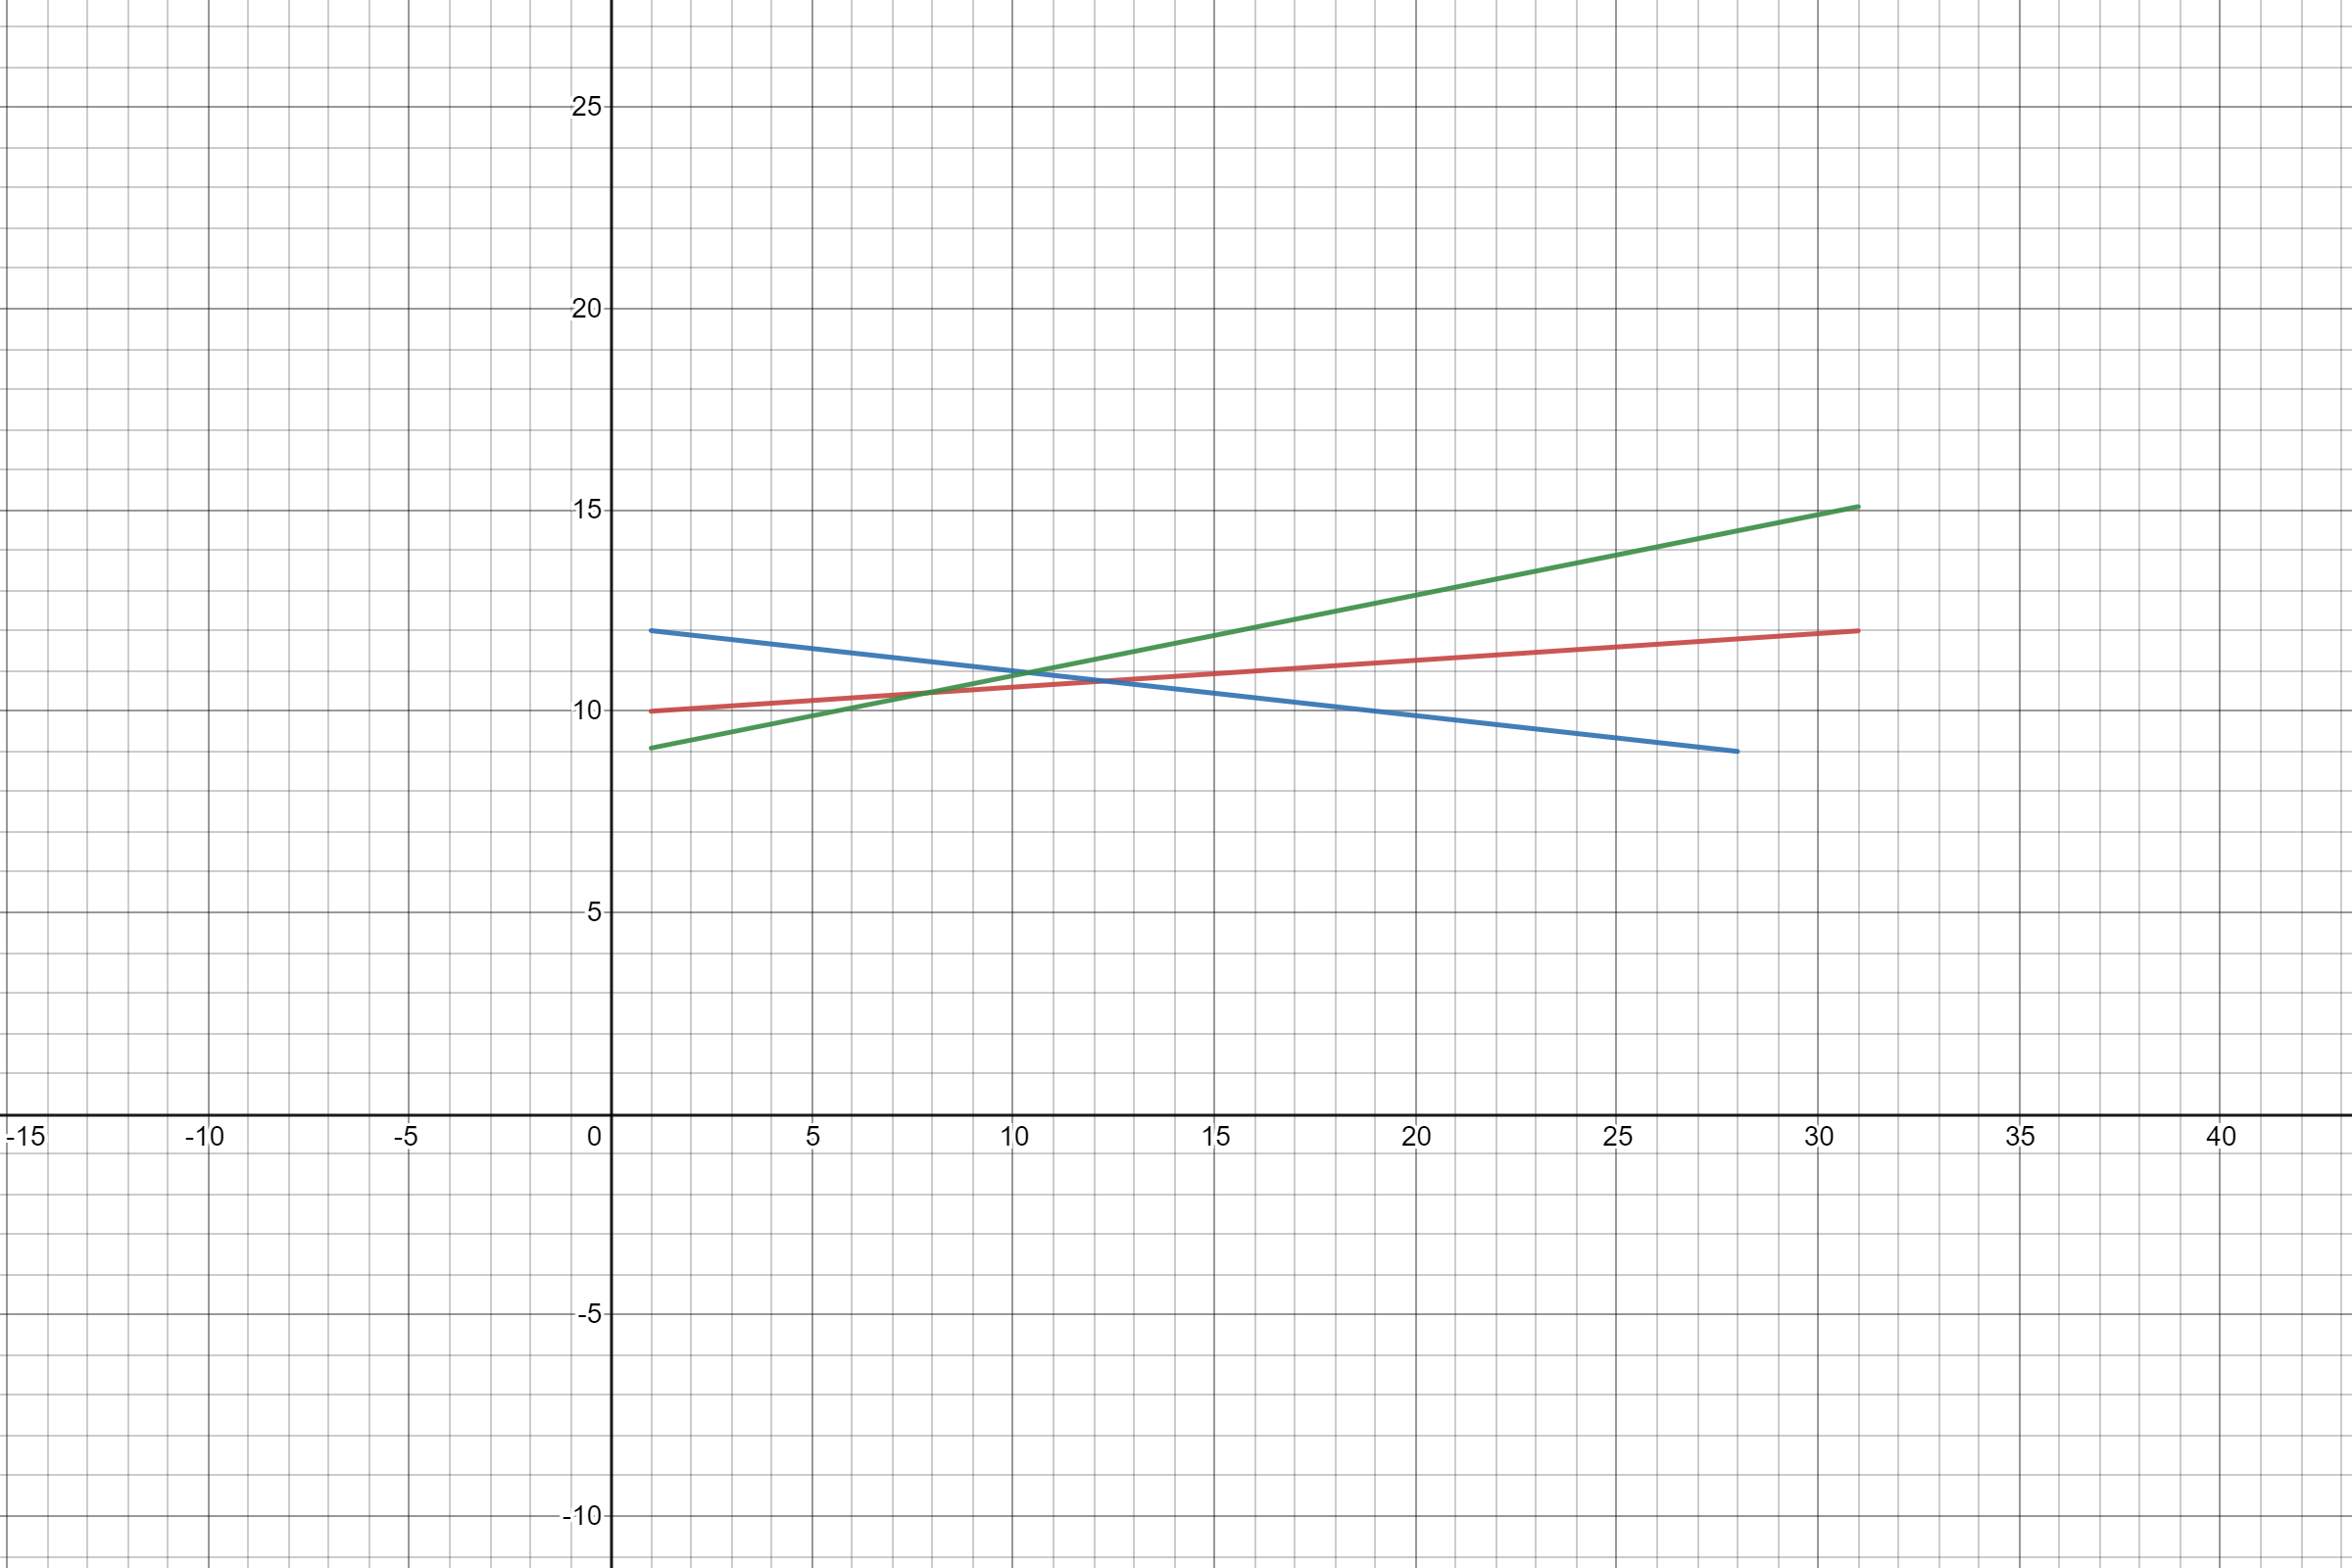
\includegraphics[scale = 0.1]{DAunit2}
    
    
    \section*{Alternative GRAPH}
    The final Equations for all three months are 
    $${y=\frac{1}{15}x + 9.93  \{1\le x \le 31\}}$$
    $${y=-\frac{1}{9}x + 12.11 \{32\le x \le 60\}}$$
    $${y=\frac{1}{5}x + 8.88   \{61\le x \le 92\}}$$
    The graph is shown below\\
    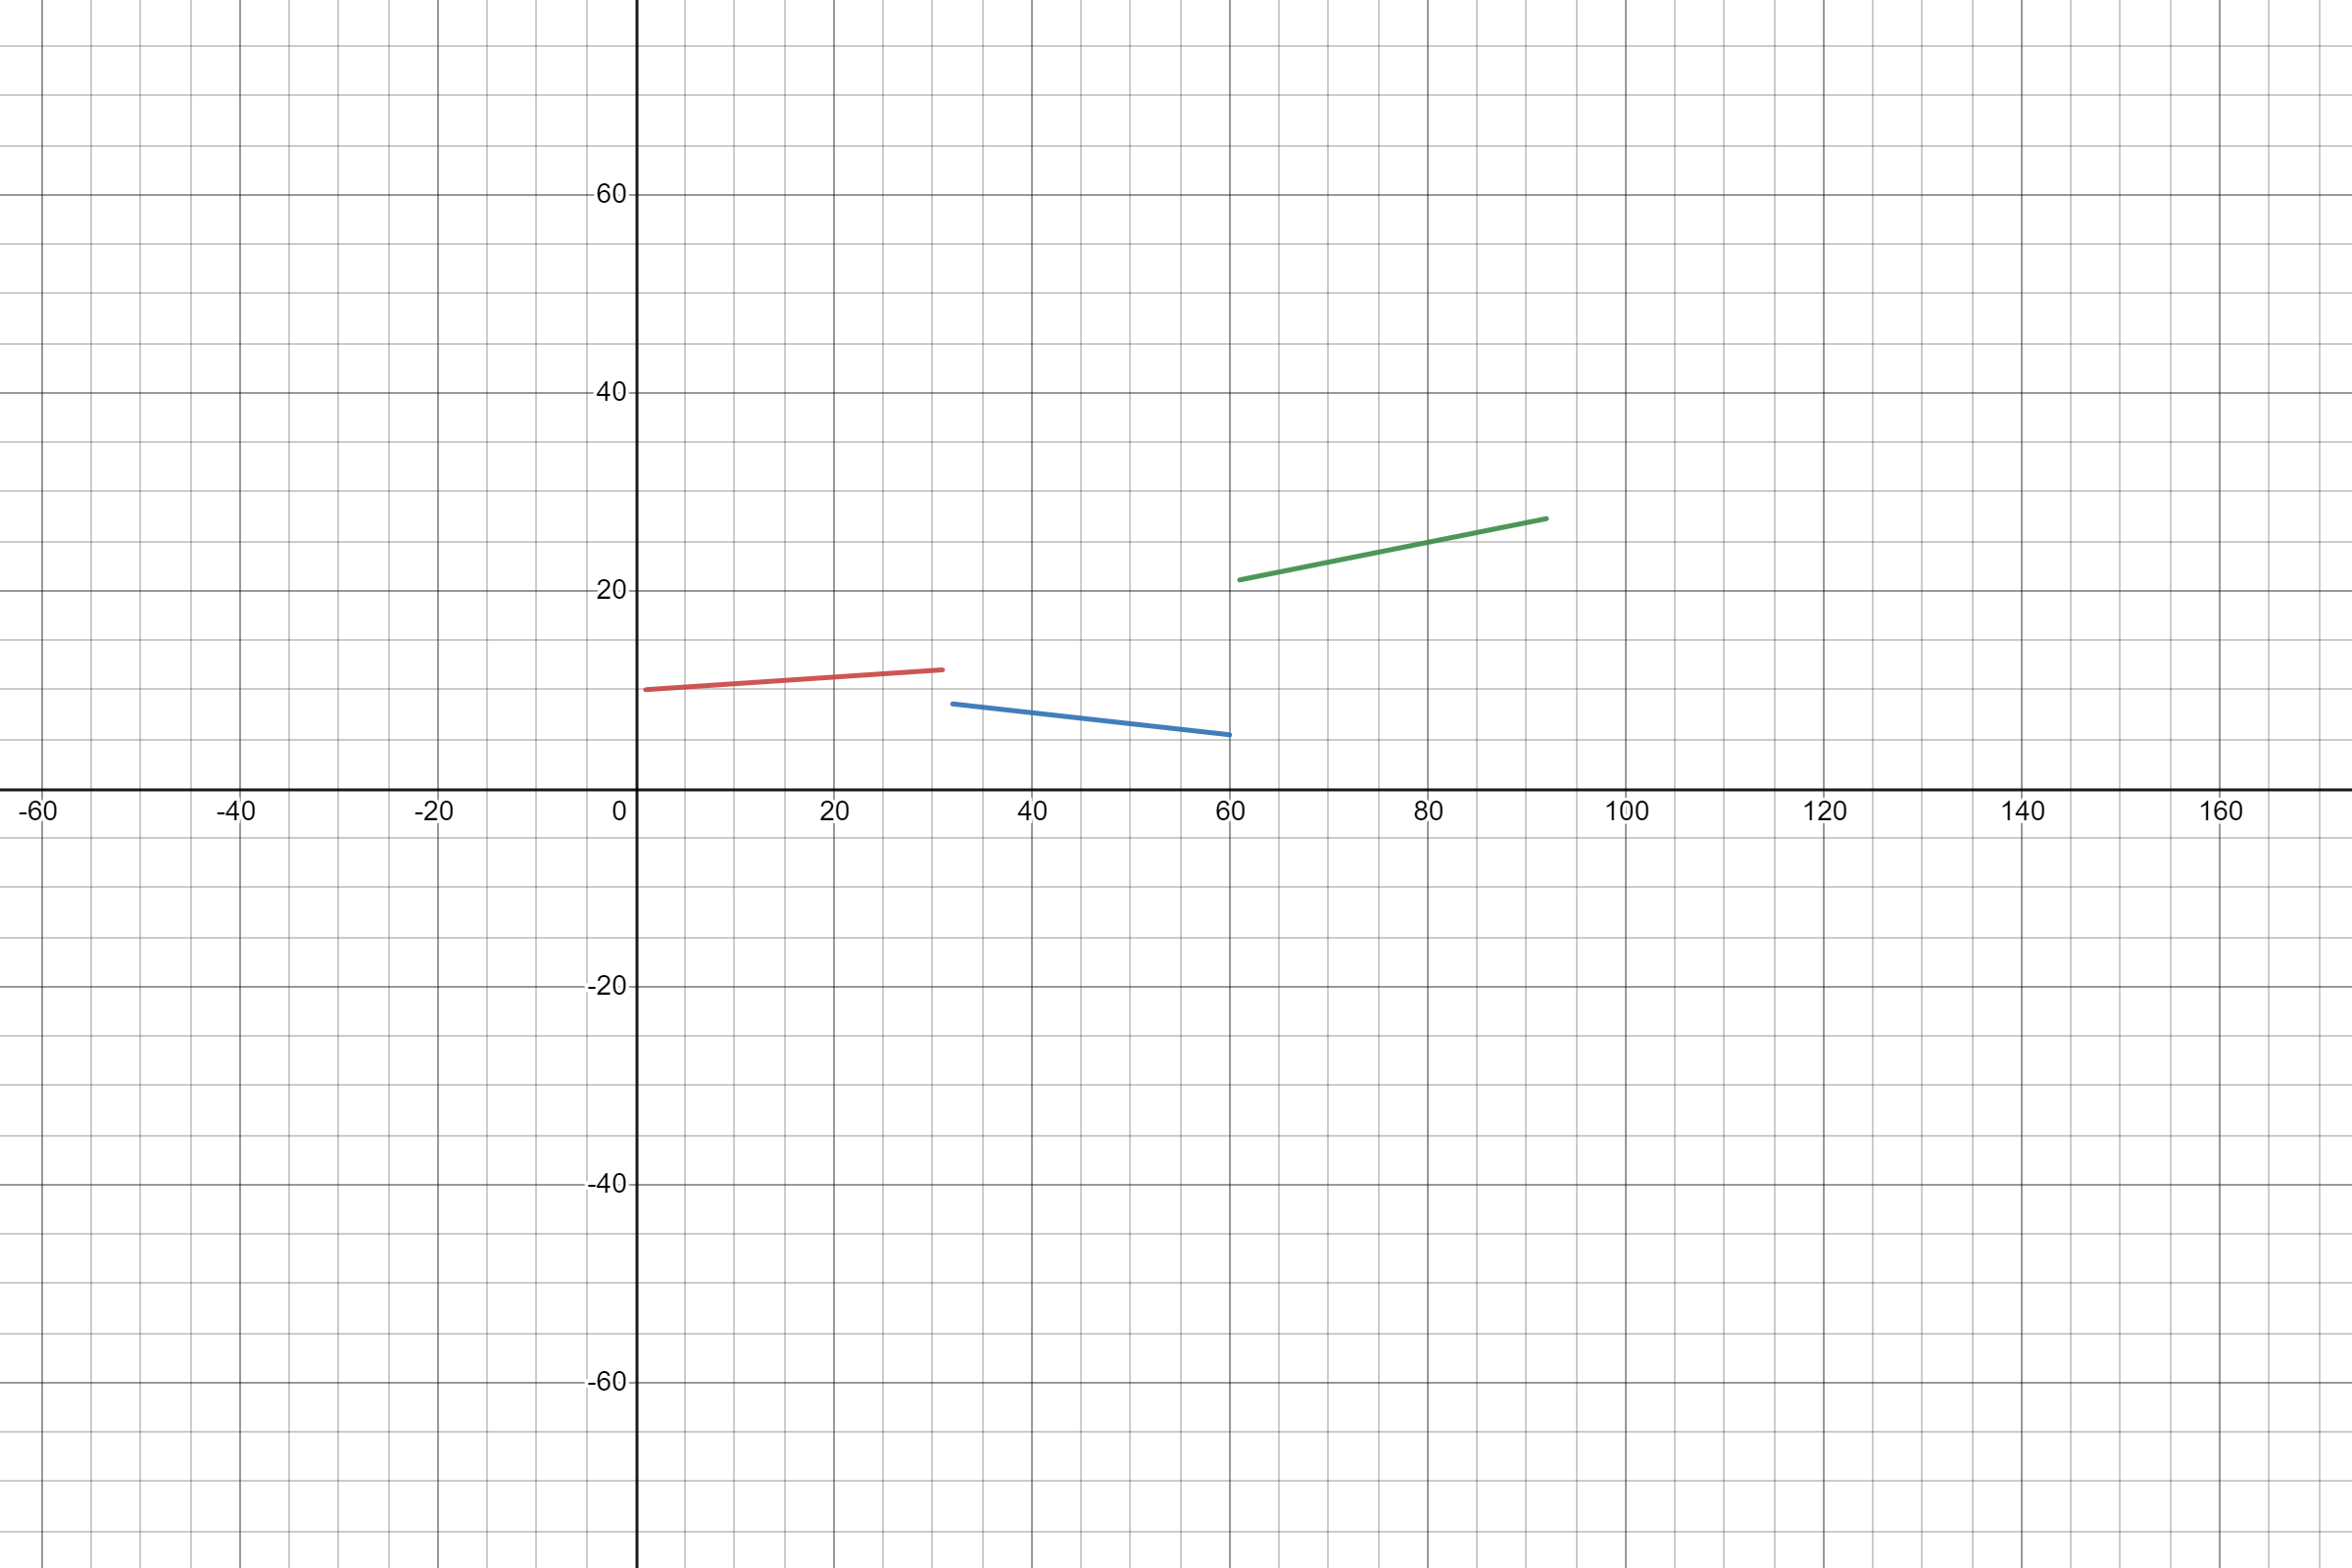
\includegraphics[scale = 0.1]{alt-graph}


    \section*{REFERENCES}
    Abramson, J. (2017). \textit{Algebra and trigonometry}. OpenStax, TX: Rice University. Retrieved from https://openstax.org/details/books/algebra-and-trigonometry

\end{itemize}

\end{document}












